\documentclass{beamer}
\usetheme{Madrid}
\usepackage{wrapfig}

\title[CQRS]{CQRS}
\author[Yan Doroshenko]{Yan Doroshenko}

\begin{document}

\frame{\titlepage}

\begin{frame}
\frametitle{What CQRS is not}

\begin{itemize}[<+->]
  \item Domain Driven Design
  \item Event sourcing
  \item Microservices
  \item Eventual consistency
  \item Framework
\end{itemize}

\end{frame}

\begin{frame}
\frametitle{What CQRS is}

\begin{itemize}
  \item<1-> Pattern
  \item<2-> Command-query request segregation

    \begin{itemize}
      \item<3-> Command (Write side)

        \only<3>{\rule{0pt}{10pt}}

        \only<3>{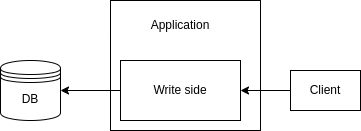
\includegraphics[width=0.4\textwidth]{img/write.png}}

      \item<4-> Query (Read side)

        \rule{0pt}{10pt}

        \only<4->{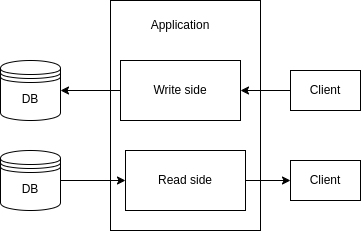
\includegraphics[width=0.4\textwidth]{img/read.png}}

    \end{itemize}
\end{itemize}

\end{frame}

\begin{frame}
\frametitle{Reasonable stack}

\begin{itemize}
  \item<1-> Event sourcing
  \item<2-> DDD
  \item<3-> Persistent message bus
  \item<4-> \only<4>{Schema evolution for events} \only<5->{Schema evolution for events (Protobuf)}
  \item<6-> Query-first databases
  \item<7-> {[Optional]} Microservices
\end{itemize}

\end{frame}

\begin{frame}
\frametitle{Disadvantages}

\begin{itemize}
  \item<1-> Eventual consistency
  \item<2-> Consolidation mechanism is required
  \item<3-> Complexity
    \begin{itemize}
      \item<4-> Design
      \item<5-> Infrastructure
      \item<6-> Running locally and debugging
      \item<7-> Deployment
    \end{itemize}
\end{itemize}

\end{frame}

\begin{frame}
\frametitle{Advantages}

\begin{itemize}[<+->]
  \item Separation of concerns
  \item Scalability
  \item Replaying journal
\end{itemize}

\end{frame}

\end{document}
